\subsection{Other Models}\label{s:other_models}

In this section, we will discuss additional models tested with \texttt{dataset\_19} and their performance.

\subsubsection{VGG16}\label{ss:vgg16}

VGG16 is a convolutional neural network model proposed by K. Simonyan and A. Zisserman from the University of Oxford in the paper "Very Deep Convolutional Networks for Large-Scale Image Recognition" \cite{simonyan_very_2015}. The model achieved state-of-the-art performance in the ImageNet Large Scale Visual Recognition Challenge (ILSVRC) 2014. It comprises 16 convolutional layers and 3 fully connected layers. The model, pre-trained on the ImageNet dataset, is readily available in the Keras library.

For our study, we utilized the VGG16 model as referenced in \cite{khaliki_brain_2024}. The architecture included a GlobalAveragePooling layer followed by dropout and dense layers activated by softmax. The Rectified Adam optimizer \cite{liu_variance_2019} was employed, with a learning rate of $0.0001$, $\beta_1$ of $0.9$, $\beta_2$ of $0.999$, and $\epsilon$ of $1e-08$. The batch size was set to 10.

The VGG16 model was trained for 100 epochs, achieving an validation accuracy of 0.7556 with a validation loss of 2.1557. Despite the high accuracy reported in \cite{khaliki_brain_2024}, this model did not outperform the previously discussed models in this study. Due to limitations in computational power and time, further optimization of this model to achieve greater accuracy was not pursued.

The results of the VGG16 model are summarized in Tables \ref{tab:vgg16_metrics} and \ref{tab:vgg16_conditions}. The tables include both the evaluation metrics and the testing conditions for clarity.

\begin{table}[H]
\parbox{.45\linewidth}{
\centering
\caption{Performance Metrics for VGG16 Model}\label{tab:vgg16_metrics}
\begin{tabular}{|l|c|c|c|c|}
\hline
\textbf{Class} & \textbf{Precision} & \textbf{Recall} & \textbf{F1-Score} & \textbf{Support} \\
\hline
meningioma & 0.95 & 0.75 & 0.84 & 24 \\
\hline
pituitary & 0.76 & 0.79 & 0.78 & 24 \\
\hline
glioma & 0.88 & 0.88 & 0.88 & 24 \\
\hline
notumor & 0.86 & 1.00 & 0.92 & 24 \\
\hline
micro avg & 0.85 & 0.85 & 0.85 & 96 \\
\hline
macro avg & 0.86 & 0.85 & 0.85 & 96 \\
\hline
weighted avg & 0.86 & 0.85 & 0.85 & 96 \\
\hline
samples avg & 0.85 & 0.85 & 0.85 & 96 \\
\hline
\end{tabular}
}
\hfill
\parbox{.45\linewidth}{
\centering
\caption{Testing Conditions for VGG16 Model}\label{tab:vgg16_conditions}
\begin{tabular}{|l|c|}
\hline
\textbf{Parameter} & \textbf{Value} \\
\hline
Batch Size & 10 \\
\hline
Image Size & 224x224 \\
\hline
Learning Rate & $0.0001$ \\
\hline
Epochs & 100 \\
\hline
Optimizer & Rectified Adam \\
\hline
\end{tabular}
}
\end{table}

\begin{figure}[H]
  \centering
  \begin{subfigure}[b]{0.2\textwidth}
    \centering
    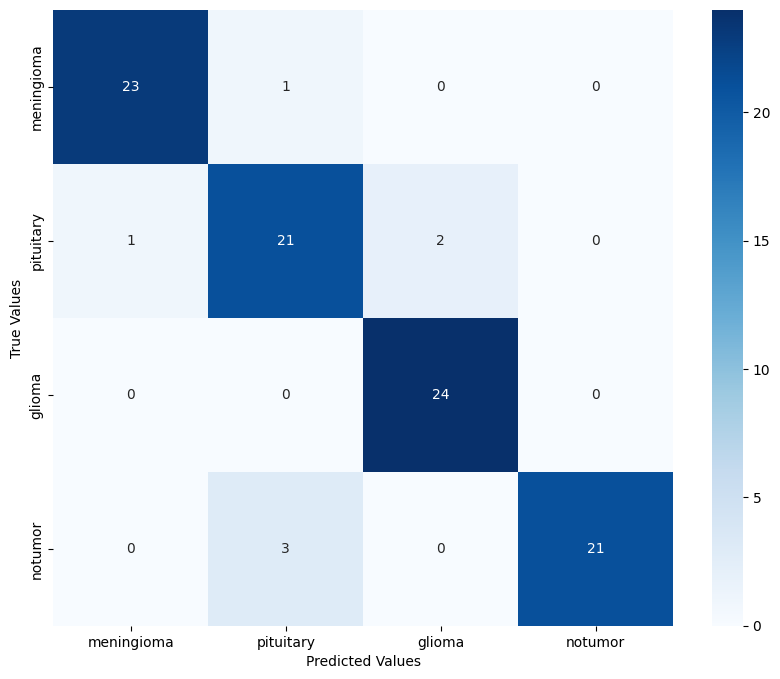
\includegraphics[width=\textwidth]{vgg16/evaluation/cm1.png}
    \caption{Confusion Matrix}
    \label{fig:vgg16_cm1}
  \end{subfigure}
  \hfill
  \begin{subfigure}[b]{0.2\textwidth}
    \centering
    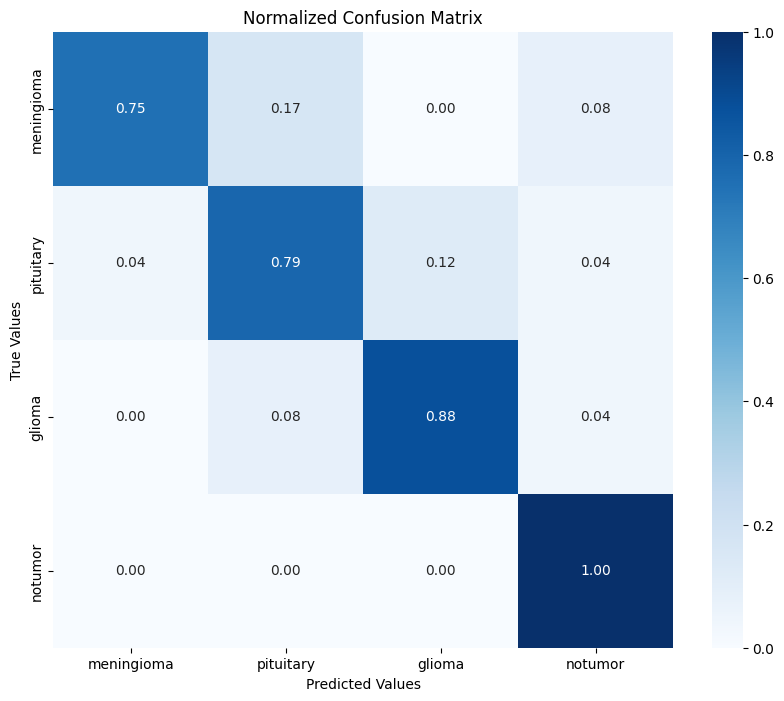
\includegraphics[width=\textwidth]{vgg16/evaluation/cm2.png}
    \caption{Normalized Confusion Matrix}
    \label{fig:vgg16_cm2}
  \end{subfigure}
  \hfill
  \begin{subfigure}[b]{0.25\textwidth}
    \centering
    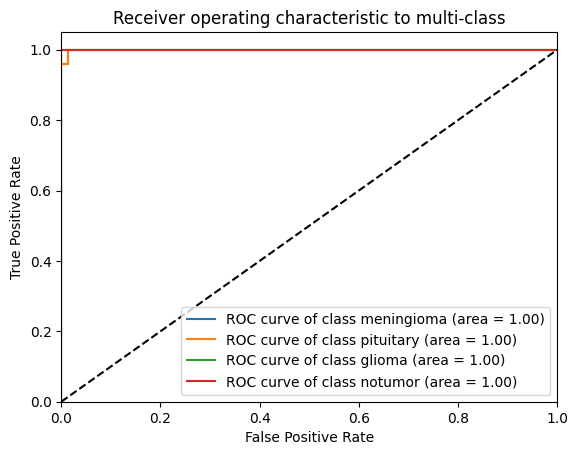
\includegraphics[width=\textwidth]{vgg16/evaluation/ROC.png}
    \caption{ROC Curve}
    \label{fig:vgg16_roc}
  \end{subfigure}
  \hfill
  \begin{subfigure}[b]{0.25\textwidth}
    \centering
    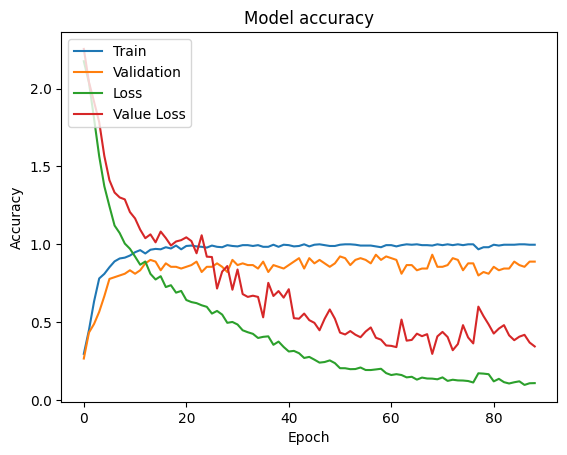
\includegraphics[width=\textwidth]{vgg16/evaluation/learning_curve.png}
    \caption{Learning Curve}
    \label{fig:vgg16_learning_curve}
  \end{subfigure}
  \caption{Confusion Matrix, Normalized Confusion Matrix, ROC Curve, and Learning Curve for Brain Tumor Segmentation}
  \label{fig:vgg16_evaluation}
\end{figure}

The evaluation of the VGG16 model highlights its decent performance with a moderate accuracy and high validation loss. These metrics suggest that while VGG16 has shown promise in previous studies, its application to our specific dataset and task did not yield superior results compared to other models. This underscores the importance of model selection based on specific task requirements and dataset characteristics. Due to the limitations of compute power and time, further optimization of this model to achieve greater accuracy was not pursued.

